\section{Missing proofs from \Cref{sec:prelims}}\label{app: missing from prelims}

\subsection{Proof of~\Cref{proposition:large-body-ball}}
    If $K$ does not contain $\varepsilon \, \Ball^d_2$, then there is $p \notin K$ such that $p \in \varepsilon \, \Ball^d_2$; therefore, since $K$ is convex, there must exist a hyperplane $h$ that separates $p$ from $K$, such that $h \cap (\varepsilon \, \Ball^d_2) \neq \emptyset$, and $h$ does not go through the origin. Denote by $H^+ \subseteq \mathbb{R}^d$ the halfspace, created by $h$, that includes the origin, and let $H^{-}$ be the other halfspace. Since $H^-$ is a halfspace that doesn't contain the origin we have that $\gamma_d(H^-) < 1/2$. Using the fact that the standard Gaussian distribution $\mathcal{N}(\mathbf{0}, \mathbf{I}^d)$ is centrally symmetric and that fact that the distance of the origin from $h$ is strictly less than $\varepsilon$, we can bound $\gamma_d(H^+) < \mathbb{P}_{u \sim \mathcal{N}(0,1)}[u \leq \varepsilon] \leq 1/2 + \varepsilon$. This leads to a contradiction, since $\gamma_d(H^+),\gamma_d(H^-) < 1/2 + \varepsilon = \gamma_d(K)$, and $K$ must lie entirely in either $H^+$ or $H^-$. \qed

\section{Missing proofs from \Cref{sec: oblivious}}\label{app: missing from section 3}

\subsection{Proof of~\Cref{theorem:tree-subgaussianity}}

We use the following proposition from~\cite{kulkarni2024optimal}, which gives a specific symmetric convex body, whose Gaussian measure is close to $1$.

\begin{proposition}[\cite{kulkarni2024optimal}]\label{proposition:convex-body}
    For any $d, N \in \mathbb{N}$, and $\delta > 0$, let 
    $K_{\delta} \coloneqq \{ (y^{(1)}, \ldots, y^{(N)}) \in \mathbb{R}^{N d}: \norm{Y}_{\psi_2,\infty} \leq 2 + \delta$, where $Y$ picks a vector uniformly at random from the set $\{y^{(1)}, \ldots, y^{(N)}\} \}$ be a symmetric convex body. For any $\delta > 0$, there exists a constant $C_{\delta} > 0$ such that for all $d,N \in \mathbb{N}$, we have $\gamma_{Nd}(K_\delta) \geq 1 - \frac{C_{\delta}^d}{N^{1+\delta}}$.
\end{proposition}



    We will construct a tree $\calT' = (V',E')$ and then invoke~\Cref{theorem:tree-reduction} using $\calT'$ and the convex body defined in~\Cref{proposition:convex-body}. To construct $\calT'$ we start with the tree $\calT = (V,E)$ and replace every $e \in E$ by a path of $N$ edges $e^{(1)}, e^{(2)}, \ldots, e^{(N)}$, for a suitable $N \in \mathbb{N}$ to be determined later in this proof; hence, we have $|E'| = N|E|$. To every edge $e^{(i)}$ we associate a set $S_e^{(i)} = \{(\mathbf{0}, \mathbf{0}, \ldots, v, \ldots, \mathbf{0}) \in \mathbb{R}^{Nd}: v \in S_e\}$ where an element/vector in $S_e^{(i)}$ can be thought of as an $N$ by $d$ matrix, where the $i^{th}$ row is a vector from $S_e$, and all other rows are $\mathbf{0}$ vectors. This completes our construction of $\calT'$. Note that, $\mathbf{0} \in \conv(S_e)$ implies that $\mathbf{0} \in \conv(S_e^{(i)})$, for all $i \in [N]$. Additionally, by Caratheodory's theorem $\mathbf{0} \in \Ball^d_2$ can be represented as a convex combination of at most $d+1$ vectors in $S_e$, which further implies that $\mathbf{0} \in \Ball^{Nd}_2$ can also be represented as a convex combination of at most $\ell = d+1$ vectors in $S^{(i)}_e$. We also consider the symmetric convex body $K_\delta$ (as defined in~\Cref{proposition:convex-body}) with $N = \left\lceil \left((d+1)C_\delta^d|E|\right)^{1/\delta}\right\rceil$ for $\delta = 0.01$. This particular choice of $N$ gives us $\gamma_{Nd}(K_\delta) \geq 1 - \frac{C_\delta^d}{N^{1+\delta}} \geq 1 - \frac{1}{(d+1)N|E|} = 1 - \frac{1}{\ell \cdot |E'|}$. 
    
    The tree $\calT'$, along with the symmetric convex body $K_\delta$, satisfy the conditions of~\Cref{theorem:tree-reduction}, and therefore for all $e \in E$ and $i \in [N]$ there exists $s^{(i)}_e \in S^{(i)}_e$ such that for all $u \in V$, $\sum_{e \in P_u} \sum_{i=1}^{N} s^{(i)}_e = \sum_{i=1}^{N} \left( \sum_{e \in P_u} s^{(i)}_e \right) \in 11 K_\delta$. From the definition of $K_\delta$ (for $\delta = 0.01$), for $v \in K$, if we view $v$ as an $N$ by $d$ matrix, the random variable that picks a row of $v$ uniformly at random is $2.01$ subgaussian. 
    For a fixed $i$, $\sum_{e \in P_u} s^{(i)}_e$ is an element of $S_e^{(i)} \subseteq \mathbb{R}^{N d}$, i.e., an $N$ by $d$ matrix with all rows equal to the $\mathbf{0}$ vector, except row $i$. And therefore, $\sum_{i=1}^{N} \left( \sum_{e \in P_u} s^{(i)}_e \right)$ can be thought of as an $N$ by $d$ matrix whose $i^{th}$ row is exactly the $i^{th}$ row of $\sum_{e \in P_u} s^{(i)}_e$. Therefore, since $\sum_{i=1}^{N} \left( \sum_{e \in P_u} s^{(i)}_e \right) \in 11 K$ for all $u \in V$, the random variable $\sum_{e \in P_u} s^{(j)}_e$ (supported on $\mathbb{R}^{Nd}$) where $j \sim \mathcal{U}([N])$ is $\left(11 \cdot 2.01 \right) = 22.11$-subgaussian. And, since all but the $i^{th}$ row of $s^{(i)}_e$ are equal to the $\mathbf{0}$ vector, we also have that the distribution $\calD$ that samples $j \sim \mathcal{U}([N])$ and then outputs the $j$-th row of $s^{(j)}_e$, for all $e \in E$, a distribution supported on $\bigtimes_{e \in E} S_e$, is also $22.11$-subgaussian. \qed

\subsection{Proof of~\Cref{lemma:weighted-vector-balancing}}
    Consider the algorithm of~\Cref{theorem:subgauss-algo} where the set at time $t$ is $S_t = \{(1-\alpha)v_t, -\alpha v_t\}$, and let $s_t \in S_t$ be the choice of this algorithm. If $s_t = (1-\alpha) v_t$, set $w_t = 1-\alpha$; otherwise, set $w_t = -\alpha$. Notice that the constant subgaussianity of $\sum_{i=1}^t s_i$ implies, by~\Cref{prop: subgaussian means small tail}, that with probability at least $1- \delta / T$, for every fixed $t$, we have $\norm{\sum_{i=1}^t s_i}_2 < 23 \sqrt{\log\left(\frac{2T}{\delta}\right)}$. Thus, taking a union bound over all $t\in [T]$, with probability at least $1-\delta$, we have $\norm{\sum_{i=1}^t w_i v_i}_\infty \leq \norm{\sum_{i=1}^t w_i v_i}_2 = \norm{\sum_{i=1}^t s_i}_2 \leq \sqrt{\log(\frac{2T}{\delta})} \leq \sqrt{\log(T)} + \sqrt{\log(\frac{2}{\delta})}$, for all $t \in [T]$ simultaneously. \qed

\subsection{Proof of Theorem~\ref{theorem:adaptive-lb}}\label{app:proof from OR paper}

In this section, we show that, for any $n \geq 2$, $r < 1$ and $T \geq 1$, in the online envy minimization problem, there exists a set of instances $S_T$, with $|S_T|  \leq 2^T$, such that, for any deterministic online fair division algorithm $\mathcal{A}$, there exists an instance $I \in S_T$, such that running algorithm $\mathcal{A}$ on the sequence of items $1,2 \ldots, T$ described by $I$ results in $\env^T \in \Omega((T/n)^{r/2})$. We first prove the bound for $n=2$, followed by the case of an arbitrary number of agents.

%\subsubsection*{Lower Bound for Two Agents}

\begin{lemma}\label{lem:LBn=2}
For $n = 2$ and any $r < 1$, there exists a set of instances $S_T$, with $|S_T|  \leq 2^T$, such that, for any online fair division algorithm $\mathcal{A}$, there exists an instance $I \in S_T$, such that running algorithm $\mathcal{A}$ on the sequence of items $1,2 \ldots, T$ described by $I$ results in $\env^T \in \Omega(T^{r/2})$.
\end{lemma}

%\proof{Proof of Lemma~\ref{lem:LBn=2}.}
\begin{proof}
We will describe a strategy for the adaptive adversary. The adversary will generate an instance overtime, as the algorithm makes its choices. The set of instances $S_T$ is the set of all possible instances; $|S_T|  \leq 2^T$ since the algorithm makes a binary choice at each step.

Label the agents $L$ and $R$, and let $\{v_0 = 1,v_1,v_2,\ldots\}$ be a decreasing sequence of values (specified later) satisfying $v_{d} - v_{d+1} < v_{d'} - v_{d'+1}$ for all $d' < d$. The adversary keeps track of the \emph{state} of the game, and the current state defines its strategy for choosing the agents' valuations for the next item. The lower bound follows from the adversary strategy illustrated in Figure~\ref{fig:LB}. Start in state $0$, which we will also refer to as $L_0$ and $R_0$, where the adversary sets the value of the arriving item as $(1,1)$. To the left of state $0$ are states labeled $L_1,L_2,\ldots$; when in state $L_d$, the next item that arrives has value $(1,v_d)$. 
To the right of state $0$ are states labeled $R_1,R_2,\ldots$; when in state $R_d$ the next item  arrives with value $(v_d,1)$. Whenever the algorithm allocates an item to agent $L$ (resp.\ $R$), which we will refer to as making an $L$ (resp.\ $R$) step, the adversary moves one state to the left (resp.\ right).

\begin{figure}[b]
        \centering
	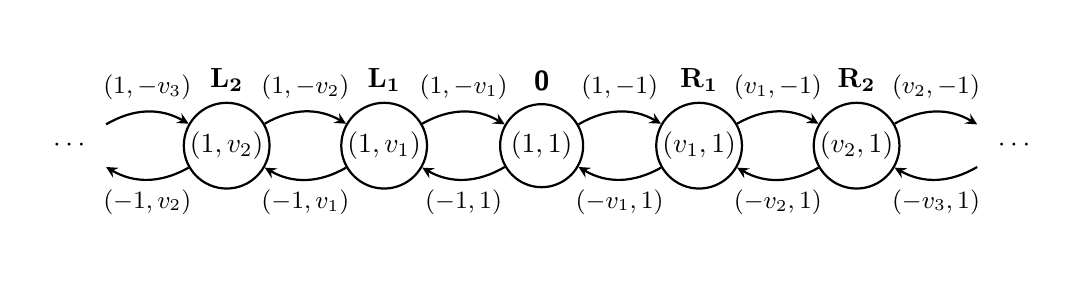
\begin{tikzpicture}[->,>=stealth,auto,node distance=2cm,
    thick,every node/.style={circle,draw,font=\sffamily,minimum size=3em,inner sep=1}]

		%
		\node [label={[label distance=-0.75em]north:{\textbf{0}}}] (0) {$(1,1)$};
		%
		\node [right of=0,label={[label distance=-0.75em]north:{$\mathbf{R_1}$}}] (1) {$(v_1,1)$};
		\node [right of=1,label={[label distance=-0.75em]north:{$\mathbf{R_2}$}}] (2) {$(v_2,1)$};
		\node [right of=2,draw=none] (3) {$\cdots$};  
		%
		\node [left of=0,label={[label distance=-0.75em]north:{$\mathbf{L_1}$}}] (-1) {$(1,v_1)$};
		\node [left of=-1,label={[label distance=-0.75em]north:{$\mathbf{L_2}$}}] (-2) {$(1,v_2)$};
		\node [left of=-2,draw=none] (-3) {$\cdots$};  
		%
		\path 
		(-3) edge [bend left] node [draw=none,label={[align=center,above=-4em]\small $(1,-v_3)$}] {} (-2)
		(-2) edge [bend left] node [draw=none,label={[align=center,above=-4em]\small $(1,-v_2)$}] {} (-1)
		(-1) edge [bend left] node [draw=none,label={[align=center,above=-4em]\small $(1,-v_1)$}] {} (0)
		(0) edge [bend left] node [draw=none,label={[align=center,above=-3.81em]\small $(1,-1)$}] {} (1)
		(1) edge [bend left] node [draw=none,label={[align=center,above=-4em]\small $(v_1,-1)$}] {}  (2)
		(2) edge [bend left] node [draw=none,label={[align=center,above=-4em]\small $(v_2,-1)$}] {}  (3);
		\path 
		(3) edge [bend left] node [draw=none,label={[align=center,below=-1em]\small $(-v_3,1)$}] {} (2)
		(2) edge [bend left] node [draw=none,label={[align=center,below=-1em]\small $(-v_2,1)$}] {} (1)
		(1) edge [bend left] node [draw=none,label={[align=center,below=-1em]\small $(-v_1,1)$}] {} (0)
		(0) edge [bend left] node [draw=none,label={[align=center,below=-0.81em]\small $(-1,1)$}] {} (-1)
		(-1) edge [bend left] node [draw=none,label={[align=center,below=-1em]\small $(-1,v_1)$}] {} (-2)
		(-2) edge [bend left] node [draw=none,label={[align=center,below=-1em]\small $(-1,v_2)$}] {} (-3);
		\end{tikzpicture}
	%\vspace{-1em}
	\caption{Adversary strategy for the two-agent lower bound. In state $L_d$, an item valued $(1,v_d)$ arrives, while in state $R_d$, an item valued $(v_d,1)$ arrives. The arrows indicate whether agent $L$ or agent $R$ is given the item in each state. The arrows are labeled by the amount envy changes after that item is allocated.}\label{fig:LB}
	%\vspace{-1.5em}
\end{figure} 


We construct the optimal allocation algorithm against this adversary, and show that for this algorithm the envy at some time step $t \in [T]$ will be at least $\Omega(T^{r/2})$ for the given $r<1$.
This immediately implies Lemma~\ref{lem:LBn=2}: if the envy is sufficiently large at any time step $t$ the adversary can guarantee the same envy at time $T$ by making all future items valued at zero by both agents.

The intuition for the adversary strategy we have defined is that it forces the algorithm to avoid entering state $L_d$ or $R_d$ for high $d$, as otherwise the envy of some agent will grow to $v_0 + v_1 + \cdots + v_d$, which will be large by our choice of $\{v_d\}$. At the same time, if an $L$ step is taken at state $L_d$, followed by a later return to state $L_d$, the envy of $R$ increases by at least $v_d-v_{d+1}$; we choose $\{v_d\}$ so that this increase in envy is large enough to ensure that any algorithm which spends too many time steps close to state $0$ incurs large envy.



By the pigeonhole principle, either the states to the left or to the right of state $0$ are visited for at least half the time.
Assume, without loss of generality, that our optimal algorithm spends time $T' = \left\lceil{T/2}\right\rceil$ in the ``left'' states ($L_0, L_1,\ldots$), and that $T'$ is even.
We prove that the envy of agent $R$ grows large at some time step $t$.
We ignore any time the algorithm spends in the states $R_d$, $d \ge 1$.
To see why this is without loss of generality, consider first a cycle spent in the right states that starts at $R_0$ with an item allocated to $R$ and eventually returns to $R_0$.
In such a cycle, an equal number of items are allocated to both agents.
All of these items have value $1$ to agent $R$, yielding a net effect of $0$ on agent $R$'s envy. ({We ignore agent $L$ completely, as our analysis is of the envy of agent $R$.}) The other case is when the algorithm starts at $R_0$ but does not return to $R_0$. This scenario can only occur once, which means that the algorithm has already taken $T'$ steps on the left side; the allocation of these items does not affect our proof.

Let  $0 \leq K \leq T'/2$ be an integer and denote by $\OPT(K)$ the set of envy-minimizing allocation algorithms that spend the $T'$ steps in states $L_0, \ldots, L_{K}$ (and reach $L_K$). Note that the algorithm aims to minimize the maximum envy at any point in its execution. 
Let $\mathcal{A}^*(K)$ be the following algorithm, starting at $L_0$:
Allocate the first $K$ items to agent $L$, thus arriving at state $L_{K}$.
Alternate between allocating to agents $R$ and $L$ for the next $T'-2K$ items, thereby alternating between states $L_{K-1}$ and $L_{K}$.
Allocate the remaining $K$ items to agent $R$. Our first result is that $\mathcal{A}^*(K)$ belongs to $\OPT(K)$.

\begin{lemma}\label{lem:lb:A*opt}
	$\mathcal{A}^*(K) \in \OPT(K)$.
\end{lemma}
 
%\begin{proof}%[Proof of Lemma~\ref{lem:lb:A*opt}.]


%{\color{red}Let us assume for now that indeed $K\leq T'/2$.} 
We analyze the envy of $\mathcal{A}^*(K)$ as a function of $K$ before optimizing $K$.
Agent $R$'s maximum envy is realized at step $T' - K$, right before the sequence of $R$ moves. $\env^{T'-K}$ has two terms: the envy accumulated to reach state $L_{K}$, and the envy from alternating $R$ and $L$ moves between states $L_{K}$ and $L_{K-1}$, so 
%$\env^{T'-K} = \sum_{d=0}^{K-1} v_d + \frac{T'-2K}{2} \cdot \left( v_{K-1}-v_{K} \right).$
%
\begin{align}
\env^{T'-K} 
= \sum_{d=0}^{K-1} v_d + \frac{T'-2K}{2} \cdot \left( v_{K-1}-v_{K} \right). \label{eq:adaptive1}
\end{align}
%
Given $r<1$, define $v_d \defeq (d+1)^r - d^r$.  Notice that $\sum_{d=0}^{K-1} v_d = K^r$. 
\edit{When  $K\geq \sqrt{T'/2}$ it follows that  $\sum_{d=0}^{K-1} v_d \geq (T'/2)^{r/2} \in \Omega(T^{r/2})$, which is what we set out to prove. We limit the rest of the analysis to the case where  $K\leq \sqrt{T'/2}$. }

%\begin{restatable}{lem}{jeefa}
%\label{lem:lb:bound-diff}
%$v_{K-1} - v_{K} \geq r (1-r) K^{r-2}$.
%\end{restatable}

\begin{lemma}
	\label{lem:lb:bound-diff}
	\edit{Let $K\leq \sqrt{T'/2}$ and define $v_d \defeq (d+1)^r - d^r$ for $r<1$.} Then $v_{K-1} - v_{K} \geq r (1-r) K^{r-2}$.
\end{lemma}

Applying Lemma~\ref{lem:lb:bound-diff}  to \eqref{eq:adaptive1} and distributing terms yields
\begin{align}
\env^{T'-K} \geq K^r - r (1-r) K^{r-1} + \frac{T'}{2} r (1-r) K^{r-2} \geq \frac{1}{2} \left( K^r + {T'} r (1-r) K^{r-2} \right), \label{eq:adaptive2}
\end{align}
where the second inequality uses the fact that $r(1-r) \le 1/4 < 1/2$ and assumes $K > 1$ (otherwise the envy would be linear in $T'$).
To optimize $K$, noting that the second derivative of the above bound is positive for $K\leq \sqrt{T'/2}$, we find the critical point:
%To optimize $K$, we find the critical point of the above bound after confirming that the second derivative is positive when $K\leq \sqrt{T'/2}$:
\begin{align*}
\frac{\partial}{\partial K} \left(K^r + {T'} r (1-r) K^{r-2}\right) = r K^{r-1} - T'r(1-r)(2-r) K^{r-3} = 0  \implies  K = \sqrt{T'(1-r)(2-r)}.
\end{align*}
Defining $C_1 \defeq \sqrt{(1-r)(2-r)}$ and  substitute  into \eqref{eq:adaptive2} to obtain
%\[
%\env^{T'-K} 
%\ge \frac{1}{2} \left(C_1^r (T')^{r/2} + T' r (1-r) C_1^{r-2} (T')^{r/2 -1} \right)
%\in \Omega(T^{r/2}). \Halmos
%\]
\begin{align}
	\env^{T'-K} 
	\ge \frac{1}{2} \left(C_1^r (T')^{r/2} + T' r (1-r) C_1^{r-2} (T')^{r/2 -1} \right)
	\in \Omega(T^{r/2}),
\end{align}
%{\color{red}
%It remains to tackle the case of $K>T'/2$. But in that case the envy (at the leftmost state that is reached) is at least $\sum_{d=0}^{K-1} v_d > (T'/2)^r\in \Omega(T^{r/2})$. 
%This completes the proof of Lemma~\ref{lem:LBn=2}.
completing the proof.
\end{proof}

The extension to $n$ agents follows from the same set of instances for agents $L$, $R$, letting all other agents value every item at zero. \qed


\section{Missing Proofs from Section~\ref{sec: iid}}\label{app:missing proofs from iid}

\subsection{Proof of \Cref{lem:no-cycle}}

    We first claim that a sufficient condition for avoiding cycles at time step $t$ is that $v_j(A^t_i)   \le v_i(A^t_i)  + c$ for all agents $i \ne j$. Indeed, consider a cycle of agents $i_1, \ldots, i_k, i_{k+1}=i_1$. Then, we have \begin{align*}
        \sum_{j = 1}^k \envy_{i_{j}, i_{j + 1}}  &= \sum_{j = 1}^k v_{i_j}(A_{i_{j + 1}}) - v_{i_j}(A_{i_j})\\
        &= \sum_{j = 1}^k v_{i_j}(A_{i_{j + 1}}) - \sum_{j = 1}^k v_{i_j}(A_{i_j})\\
        &= \sum_{j = 1}^k v_{i_j}(A_{i_{j + 1}}) - \sum_{j = 1}^k v_{i_{j+1}}(A_{i_{j+1}})\\
        &= \sum_{j = 1}^k v_{i_j}(A_{i_{j + 1}}) - v_{i_{j + 1}}(A_{i_{j + 1}})\\
        &\le k \cdot c.
    \end{align*}
    Thus, for at least one pair, $\envy^t_{i_j, i_{j + 1}} \le c$, preventing a cycle from forming.

    Now, fix two agents $i \ne j$. We aim to show that
    \[
        \Pr[\forall t \ge T^{(1)}, \, v_i(A^t_i) -  v_j(A^t_i) < - c] \le 4 \cdot \left(\frac{8 e n^2 \log T}{\sqrt{T}} \right)^{c + 1}. 
    \]
    Applying a union bound over the $n(n - 1)$ pairs of $i$ and $j$ yields the lemma statement.

    Without loss of generality, we relabel $i = 1$ and $j = 2$. Define $Z_t := v_1(A^t_1) - v_2(A^t_1)$ as the difference in values at time $t$. Our goal is to show that $Z_t \ge -c$ for all $t \ge T^{(1)}$ with high probability.

    We decompose $A^t_1$ into the portion received during each phase:
    \[
        v_1(A^t_1) - v_2(A^t_1) = v_1(A^t_1 \cap G^{welf} ) - v_2(A^t_1 \cap G^{welf} ) + v_1(A^t_1 \setminus G^{welf}) - v_2(A^t_1 \setminus G^{welf}). 
    \]
    Since $t \ge T^{(1)}$, we can express 
    \[
         v_1(A^t_1 \cap G^{welf} ) - v_2(A^t_1 \cap G^{welf} ) = \sum_{j = 1}^{T^{(1)}} \left(V^{g^{welf}_j}_1 - V^{g^{welf}_j}_2 \right)  \cdot \mathbb{I}[g^{welf}_j \in A^t_1].
    \]
    Define \[X_j = \left(V^{g^{welf}_j}_2 - V^{g^{welf}_j}_1 \right)  \cdot \mathbb{I}[g^{welf}_j \in A^t_1].\]
    Now, consider $A^t_1 \setminus G^{welf}$. By \Cref{lem:phase-2-items}, we have that \[|A^t_1 \setminus G^{welf}| \le (n - 1) \cdot \ceil{\log T \sqrt{T}}.\] 
    Thus, we have $A^t_1 \setminus G^{welf} \subseteq \{g^1_1, \ldots, g^1_{(n - 1) \cdot \ceil{\log T \sqrt{T}}} \}$ (recall our way of sampling an instance). Furthermore, we can lower-bound 
    \[v_1(A^t_1 \setminus G^{welf}) - v_2(A^t_1 \setminus G^{welf}) \ge -  \sum_{j = 1}^{(n - 1) \cdot \ceil{\log T \sqrt{T}}} (V^{g^i_j}_2 - V^{g^i_j}_1)_+\] where $(s)_+ = \max(s, 0)$. That is, in this lower bound we only count items where agent $2$ had a higher value than agent $1$. Let $Y_j = (V^{g^i_j}_1 - V^{g^i_j}_2)_+$.
    
    Since the above bounds are independent of $t$, it suffices to show that $$\sum_{j = 1}^{T^{(1)}} X_j - \sum_{j = 1}^{(n - 1) \ceil{\log T \sqrt{T}}} Y_j \ge -c$$  with high probability, ensuring the bound holds for all remaining $t > T^{(1)}$.

    If $X_j$ stochastically dominated $Y_j$, then a straightforward application of~\Cref{lem:concentration} would imply the statement. Unfortunately, this is not the case. So, instead, we define the following random variables, $X'_j$, that are large sums of $X_j$ random variables, and such that the stochastic dominance we want is true. For each $j \le \floor{T^{(1)}/(2n)}$, let $X'_j = \sum_{j' = (j - 1) \cdot 2n + 1}^{j \cdot 2n} X_j$, i.e., each $X'_j$ is the sum of a distinct set of $2n$ $X_j$s. We will show that  $$\sum_{j = 1}^{\floor{T^{(1)}/(2n)}} X'_j - \sum_{j = 1}^{(n - 1) \ceil{\log T \sqrt{T}}} Y_j \ge -c$$  with high probability.
    Specifically, we will show that each $X'_j$ first-order stochastically dominates each $Y_j$. Then, by applying~\Cref{lem:concentration} we have 
    \[
    \Pr \left[ \sum_{j = 1}^{\floor{T^{(1)}/(2n)}} X'_j - \sum_{j = 1}^{(n - 1) \ceil{\log T \sqrt{T}}} Y_j < -c \right] \leq 4 \cdot \left(\frac{2 e L}{K} \right)^{c + 1},
    \]
    where $K = \floor{\frac{T - \frac{n(n-1)}{2}\ceil{\log T \sqrt{T}}}{2n}} + (n - 1) \ceil{\log T \sqrt{T}} \geq \frac{T}{2n}$ (as long as $\ceil{\log T \sqrt{T}}(\frac{3n}{4} - \frac{3}{4}) \geq 1$, which holds for $T \geq 4$), and $L = (n - 1) \ceil{\log T \sqrt{T}} \leq 2n \log T \sqrt{T}$. Note that, indeed, $\frac{K}{L} \geq \frac{\sqrt{T}}{4 n^2 \log T } \geq 4e$, for $T \in \Omega(n^6)$.
    So, overall:
    \[
    \Pr \left[ \sum_{j = 1}^{\floor{T^{(1)}/(2n)}} X'_j - \sum_{j = 1}^{(n - 1) \ceil{\log T \sqrt{T}}} Y_j < -c \right] \leq 4 \cdot \left(\frac{8 e n^2 \log T}{\sqrt{T}} \right)^{c + 1}.
    \]


    To analyze this probability, we characterize the distributions of each $X_j$, $X'_j$, and $Y_j$. We will use $X$, $X'$, and $Y$ as random variables with the same distribution as each $X_j$, $X'_j$, and $Y_j$, respectively. Recall, a way to sample $X$ is to sample $n$ values $V_1, \ldots, V_n \stackrel{\text{i.i.d.}}{\sim} \mathcal{D}$, and if $V_1$ is the largest (breaking ties randomly), set $X = V_1 - V_2$, otherwise set $ X = 0$. To define $X'$ we sum $2n$ draws from $X$. Finally, a way to sample $Y$ is to sample $n$ values $V_1, \ldots, V_n \stackrel{\text{i.i.d.}}{\sim} \mathcal{D}$ and if $V_1 \ge V_2$ (breaking ties randomly), set $Y = V_1 - V_2$, otherwise set $Y = 0$.

    All of these can be understood using distributions induced by the difference of order statistics. More formally, let $\mathcal{D}^{(k) - (\ell)}$ be the distribution obtained by drawing $V_1, \ldots, V_n \stackrel{\text{i.i.d.}}{\sim} \mathcal{D}$, sorting them as $V^{(1)} \le \cdots \le V^{(n)}$, and returning $V^{(k)} - V^{(\ell)}$.
    \begin{enumerate}
        \item  The distribution of $X$ corresponds to selecting distinct indices $i_1, i_2$ uniformly from $[n]$, and if $i_1 = n$, sampling from $\mathcal{D}^{(n) - (i_2)}$; otherwise, outputting $0$. 
        \item The distribution of $Y$ corresponds to selecting distinct indices $i_1, i_2$ uniformly from $[n]$, and if $i_1 > i_2$, sample from $\mathcal{D}^{(i_1) - (i_2)}$; otherwise, outputting $0$. 
    \end{enumerate}

The distribution of $X'$ can be described as follows:
    \begin{enumerate}
        \item Sampling $2n$ pairs $(i^j_1, i^j_2)_{j = 1, \ldots, 2n}$, where $i^j_1 \neq i^j_2$ for all $j$, from $[n]$, uniformly at random.
        \item For each pair where $i^j_1 = n$, draw a value from $\calD^{(n) - (i^j_2)}$
        \item Output the sum of these values (or output $0$ if no $i^j_1 = n$).
    \end{enumerate} 

    It remains to show that $X'$ first-order stochastically dominates  $Y$. To this end, note that if $i'_1 \ge i_1$ and $i'_2 \le i_2$, then $\mathcal{D}^{(i'_1) - (i'_2)}$ first-order stochastically dominates $\mathcal{D}^{(i_1) - (i_2)}$. We now present a sequence of distributions, each distribution stochastically dominating the previous distribution in the sequence, beginning with $Y$ and ending with $X'$. 

    

    \paragraph{Distribution 1.} We begin with the distribution of $Y$. Recall that this can be described as: draw a distinct pair $i_1, i_2 \in [n]$. If $i_1 > i_2$, sample from $\calD^{(i_1) - (i_2)}$; otherwise, output $0$. Since each ordering of $i_1$ and $i_2$ are equally likely, an equivalent description is draw a distinct pair $i_1, i_2 \in [n]$. With probability $1/2$, output $0$, and otherwise, sample from $\calD^{(\max(i_1, i_2)) - (\min(i_1, i_2))}$.

    \paragraph{Distribution 2.} With probability $1/2$, output $0$. Otherwise, sample a distinct pair $i_1, i_2$ from $[n]$ and output $\mathcal{D}^{(n) - (\min(i_2, i'_2))}$. This stochastically dominates distribution $1$ because $n \ge \max(i_1, i_2)$.

    \paragraph{Distribution 3.} With probability $1/2$, output $0$. Otherwise, sample two (not necessarily distinct) values $i_2, i_2'$ uniformly from $[n-1]$ and output $\mathcal{D}^{(n) - (\min(i_2, i'_2))}$. To show that this stochastically dominates Distribution 2,  observe that taking the minimum of a distinct pair from $[n]$ stochastically dominates taking the minimum of a (not necessarily distinct) pair from $[n - 1]$, so this only increases the likelihood of drawing from a ``better'' distribution. Specifically, the probability that $\min(i_1, i_2) \ge k$, where $i_1, i_2$ are a distinct pair from $[n]$,  is $\frac{n - k + 1}{n} \cdot \frac{n - k}{n - 1}$. The probability that $\min(i_1, i_2) \ge k$, where $i_1, i_2$ are a (possibly non-distinct) pair from $[n-1]$, is $\left(\frac{n - k}{n - 1}\right)^2$. Since $\frac{n - k + 1}{n} \, \frac{n - k}{n - 1} > \left( \frac{n - k}{n - 1} \right)^2$, the former probability is greater. As this holds for all $k$, stochastic dominance is implied.

    \paragraph{Distribution 4.} Draw $2n$ pairs $(i^j_1, i^j_2)_{j = 1, \ldots, 2n}$, where numbers in a pair are distinct, and $i^j_{\ell}$ is drawn from $[n]$. If exactly zero or exactly one pairs have $i^j_1 = n$, output $0$. Otherwise, let  $(i_1, i_2)$ and $(i'_1, i'_2)$ be the first two pairs with $i_1 = i'_1 = n$, and draw from $\mathcal{D}^{(n) - (\min(i_2, i'_2))}$. Note that conditioned on $i_1 = n$, $i_2$ is just a uniform draw from $[n - 1]$. So to establish stochastic dominance over Distribution 3, we simply need to show that the probability of at least two pairs with $i^j_1 = n$ is at least $1/2$. The number of such pairs follows a $\text{Bin}(2n, 1/n)$ distribution, which has mean $2n/n = 2$. Furthermore, it is known that the median is at least the floor of the mean~\cite{kaas1980mean}, thus, the probability of having at least two pairs is at least $1/2$, as needed.

     \paragraph{Distribution 5.} Next, we consider a distribution that only keeps the ``best'' pair.  That is, we draw $2n$ pairs  $(i^j_1, i^j_2)_{j = 1, \ldots, 2n}$ as in Distribution 4, and among those where $i^j_1 = n$, select the minimal $i^j_2$, and output $\mathcal{D}^{(n) - (i^j_2)}$ (or $0$ if no such pair exists). This stochastically dominates Distribution 4 because, in the cases when there are at least two pairs with $i^j_1 = n$, we are taking the minimum over even more values; and we are now potentially achieving a positive value even when there is only one pair with $i^j_1 = n$.

     \paragraph{Distribution 6.} Draw $2n$ pairs $(i^j_1, i^j_2)_{j = 1, \ldots, 2n}$ as in Distribution 5, and for each pair where $i^j_1 = n$, draw a value from $\calD^{(n) - (i^j_2)}$, and output the sum of these values (or output  $0$ if no $i^j_1 = n$). Note that we are only including more pairs than Distribution 5, so this stochastically dominates it. Furthermore, this is exactly the distribution of $X'$.  

     This completes the proof. \qed
    

    
    % Let $X_t$ be the contribution of good $g_t$ to $Z_t$, i.e.,
    % \[X_t = 
    %     \begin{cases}
    %         v_{2, t} - v_{1, t} & \text{if } g_t \in A^t_2\\
    %         0 & \text{otherwise.}
    %     \end{cases}
    % \]

        % WLOG $i = 1$ and $j = 2$.
        % We show in the theorem proof later that each agent receives at most $(n - 1)K$ items in phase 2 deterministically, so we will assume this to be true.

        % As before, let $S_t := v_1(A_1^t) - v_2(A_1^t)$ be the difference in values at time $t$. Our goal is to show that $S_t \ge -c$ with high probability at every step.

% Let $X_t$ be contribution to $S_t$ of good $g_t$, so $$X_t = \begin{cases}
%     v_{1t} - v_{2t} & \text{ if } g_t \in A_1^t\\
%     0 & \text{ otherwise }
% \end{cases}.$$
% We can write $S_t = \sum_{t' = 1}^t X_{t'}$. Now, it is still true that for each of the at most $(n - 1)K$ items in phase $2$, their contribution to $S_t$ stochastically dominates $\dist^{gap0}$.

% Now, for $X_t$ in phase $1$, its distribution is the following. Considering the agents ordered by their value $i$. Note that each ordering is equally likely. An item will have nonzero $X_t$ only if agent $1$ has the highest value. Thus, the distribution is $X_t = \frac{n - 1}{n} \mathbf{0} + \frac{1}{n(n - 1)} \sum_{i = 1}^{n - 1} \dist^{n:n - n:i}$. In other words, with probability $\frac{n - 1}{n}$, it is $0$, and with probability $1/(n(n-1))$, it is the difference between the $n$'th and $i$'th order statistic for each $i = 1,\ldots, n-1$. The key observation we will use is that the sum of $n(n-1)$ independent draws of these stochastically dominates $\dist^{gap0}$. Indeed, $\dist^{gap0} = 1/2 \cdot \mathbf{0} + 1/2 \dist^{2:2 - 2:1}$. Note that $\dist^{n:n - n:1}$ stochastically dominates $\dist^{2:2 - 2:1}$. In $n(n-1)$ draws, with probability at least $1 - (1 - 1/(n(n-1)))^{n(n-1)} \ge 1/2$, one of the items will follow this distribution, and all others will be nonnegative. Hence, $S_{T^{(1)}}$ stochastically dominates the sum of $T^{(1)} / (n(n-1))$ draws from $\dist^{gap0}$.
% By \Cref{lem:concentration}, we get that this occurs with probability at most $\left(\frac{2e (n - 1)n(n-1) K}{T} \right)^c \le \left(\frac{2e n^3 K}{T} \right)^c$.
    

\subsection{Proof of \Cref{lem:concentration}}

	A key observation is that, since the $Y_i$'s are i.i.d.\@ draws, by symmetry, the probability of the event we care about is equal to
	\[
		\Pr\left[\sum_{i \notin S} Y_{i} - \sum_{i  \in S} Y_{i} < -c\right],
	\]
	where $S \subseteq [K]$ is a randomly sampled set of indices of size $L$. Condition on the set of draws $Y_1, \ldots, Y_K$ having arbitrary values $y_1, \ldots, y_K$, and consider the randomness over the set $S$. By symmetry, it is without loss of generality that $y_1 \ge \cdots \ge y_K$.

    Now, by \Cref{lem:halls}, a sufficient condition for $\sum_{i \notin S} y_i + \sum_{i \in S} y_i \ge -c$ is that for all $j \in S$, $$|\{j' \in S \mid y_{j'} \ge y_j\}| \le |\{j' \notin S\mid y_{j'} \ge y_j\}| + c.$$
    A sufficient condition for this is that for all $j \le K$, $$|[j] \cap S| \le |[j] \setminus S| + c,$$ i.e., in any prefix there are the number of indices in $S$ never exceeds those outside of $S$ by more than $c$. Finally, observe that $|[j] \setminus S| = j - |[j] \cap S|$, we can again reformulate this as for all $j \le K$,
    \[
        |[j] \cap S| \le \frac{j + c}{2}.
    \]
	
	Let $\mathcal{E}^j$ be the event that $|[j] \cap S| > \frac{j + c}{2}.$ We will upper bound each $\Pr[\mathcal{E}^j]$ and then union bound  over all $j$. 
	
	Let $Z_i := \mathbb{I}[i \in S]$, so $|[j] \cap S| = \sum_{i = 1}^j Z_i$. 
    The $Z_i$s are not independent, but they \emph{are} negatively associated, and thus, traditional Chernoff bounds apply~\cite{dubhashi2009concentration}. We have  that $\mathbb{E}[Z_i] = \frac{L}{K}$ for each $i$. For $j \le c$, note that $\Pr[\mathcal{E}^j] = 0$ because $\sum_{i=1}^j Z_i \le j \le \frac{j + c}{2}$. For $j \ge c + 1$, note that $\mathbb{E}[\sum_{i = 1}^j Z_i]$ is precisely $\mu := \frac{j \cdot L}{K}$. We would like to upper bound the probability that $\sum_{i = 1}^j Z_i$ exceeds $\frac{j + c}{2}$. Since the $Z_i$s are integral, it suffices to bound the probability that  $\sum_{i = 1}^j Z_i$ exceeds $\ceil*{\frac{j + c}{2}}$. Let $\delta$ be such that  $\ceil*{\frac{j + c}{2}} = (1 + \delta) \mu$. Note that since $L/K \le 2$, $\mu \le j/2$, and therefore, $\delta > 0$. Furthermore, $$1 + \delta = \frac{j + c}{2 \mu} \ge \frac{j}{2\mu} =  \frac{K}{2 L}.$$ Using the Chernoff bound, we have:
	\[
		\Pr[X \ge (1 + \delta) \mu] \le \left(\frac{e^\delta}{(1 + \delta)^{1 + \delta}} \right)^\mu \leq  \left(\frac{e}{(1 + \delta)} \right)^{(1 + \delta)\mu} \le  \left(\frac{2 e L}{K} \right)^{\ceil*{\frac{j + c}{2}}}.
	\]
	
	Applying a union bound over all $j$, we have that
\begin{align*}
    \Pr\left[\bigcup_{j \le K} \mathcal{E}^j \right]
    &\le \sum_{j = 0}^K \Pr[\mathcal{E}^j]\\
    &= \sum_{j = c + 1}^K \Pr[\mathcal{E}^j]\\
    &\le \sum_{j = c + 1}^K \left(\frac{2 e L}{K} \right)^{\ceil*{\frac{j + c}{2}}}\\
    &\le \sum_{j = c + 1}^\infty \left(\frac{2 e L}{K} \right)^{\ceil*{\frac{j + c}{2}}}\\
    &\le \sum_{j = 0}^\infty \left(\frac{2 e L}{K} \right)^{\ceil*{\frac{j + 2c + 1}{2}}}\\
    &\le \sum_{j = 0}^\infty \left(\frac{2 e L}{K} \right)^{\ceil*{\frac{2j + 2c + 1}{2}}} + \left(\frac{2 e L}{K} \right)^{\ceil*{\frac{2j + 1 + 2c + 1}{2}}}\\
    &= \sum_{j = 0}^\infty 2 \left(\frac{2 e L}{K} \right)^{j + c + 1}\\
    &= 2 \left(\frac{2 e L}{K} \right)^{c + 1} \cdot \sum_{j = 0}^\infty \left(\frac{2 e L}{K} \right)^{j}\\
    &= 2 \left(\frac{2 e L}{K} \right)^{c + 1} \cdot \frac{1}{1 - \frac{2eL}{K}}\\
    &\le 4  \left(\frac{2 e L}{K} \right)^{c + 1},
\end{align*}
where the last two transitions use the fact that $\frac{2eL}{K} \le 1/2$. \qed

\subsection{Proof of \Cref{lem:phase-2-items}}
We will prove this by induction on the time steps. Note that at $T^{(1)}$, no phase 2 items have been given out, so $w^t_{i} = 0$ for all $i$, satisfying the lemma statement. Now suppose this is true at some fixed time $t$, and suppose the current sorted vector is $(w^t_{i_1}, \ldots, w^t_{i_n})$. Importantly, the sorted vector after the item has been given can be obtained by incrementing one entry. Specifically, the sorted vector will become $(w^t_{i_1}, \ldots, w^t_{{i_j}} + 1, \ldots  w^t_{i_n})$ where $i_j$ is the maximal $j$ such that the receiving agent had $w^t_{{i_j}}$ items. If $j = 1$ (the item was given to the agent with the fewest items), the inductive hypothesis clearly holds. We simply need to show that $w^t_{{i_{j - 1}}} \ge w^t_{{i_j}} - \ceil{ \log T \sqrt{T}}$. Importantly, the agent receiving the item $i$ must have $i \in S$, as defined on line 5. Thus $\{i_1, \ldots, i_j\} \subseteq S$ because each of these agents have currently received at most $i_j$ items. Furthermore, $w^t_{{i_{j - 1}}} \ge w^t_{{i_j}} - \ceil{ \log T \sqrt{T}}$, as otherwise $\{i_1, \ldots, i_{j - 1}\}$ satisfies the condition of line 5, and is strictly smaller in cardinality than the chosen $S$. Therefore, even after this addition $w^t_{{i_j}} + 1 - w^t_{{i_{j - 1}}} \le \ceil{ \log T \sqrt{T}}$.

To establish the general upper bound of $w^t_{i_n} \le (n - 1) \ceil{\log T \sqrt{T}}$, suppose for a contradiction there was a time step $t > T^{(1)}$ where $w_{i_n} > (n-1) \ceil{\log T \sqrt{T}}$. Then, by a straightforward induction over $j$, \[w_{i_{n + 1 - j}} > (n - j) \cdot \ceil{\log T \sqrt{T}},\] for all $1 \le j \le n$. Summing over all agents implies that phase 2 must last $> \frac{n(n - 1)}{2} \cdot \ceil{\log T \sqrt{T}}$. This is a contradiction.\qed

\subsection{Proof of \Cref{lem:halls}}
Fix values $a_1, \ldots, a_k$ and $b_1, \ldots, b_\ell$. Consider a bipartite graph with nodes $[k]$ on the left side and nodes $[\ell]$ on the right. We will have an edge $(i, j)$ precisely when $a_i \le b_j$. We would like to show that there is a matching in this graph of size at least $k - c$.

We first show that this is sufficient to imply the lemma. Let $M_L, M_R$ be the set of matched nodes and $U_L, U_R$ be the set of unmatched nodes on the left and right. We have that $\sum_{i \in M_L} a_i \le \sum_{i \in M_R} b_i$ by definition of the matching. Furthermore, $|U_L| \le c$, so $\sum_{i \in U_l} a_i \le c$. Putting this together, we have
\[
    \sum_i a_i = \sum_{i \in M_L} a_i + \sum_{i \in U_L} a_i \le \sum_{i \in M_R} b_i + c \le \sum_i b_i + c.
\]

To prove the existence of such a matching, it is sufficient so show that for all sets $S \subseteq [k]$, $|N(S)| \ge |S| - c$ where $N(S)$ is the neighborhood of $S$, i.e., all nodes in $[\ell]$ adjacent to at least one node in $S$~\cite{lovasz2009matching}. Fix such an $S$. Let $i \in \argmin_{i' \in S} a_{i'}$. Note that $S \subseteq \{i' \mid a_{i'} \ge a_i\}$ and $N(S) \supset \{i' \mid b_{i'} \ge a_i\}$, as all such nodes are adjacent to $a_i$. Thus, by the lemma condition $|S| \le |N(S)| + c$, as needed. \qed



\subsection{Proof of \Cref{lem:high-value-n}}

        Fix agents $i \ne j$. We will prove the statement is true for this pair of agents and then union bound over the at most $n(n - 1)$ pairs to yield the lemma statement. Without loss of generality, we will relabel $i$ as agent $1$ and $j$ as agent $2$. We will also assume $T$ is sufficiently large such that $T^{(1)} \ge T / 2$ and $\log T \sqrt{T} > 1$. The latter implies that $\ceil{\log T \sqrt{T}} \le 2 \log T \sqrt{T}$. 

        % In this analysis, instead of considering the exact values of each item, we will work with \emph{quantiles}. In particular, welfare maximization with random tie-breaking is equivalent to \emph{quantile maximization}: Quantiles for each agent are drawn i.i.d. from $\mathcal{U}[0, 1]$, and the item is given to the agent with the largest quantile, breaking ties arbitrarily (ties occur with probability $0$).

        % The set of goods $G$ is partitioned into three parts: The first $T^{(1)}$ that are allocated via quantile maximization, denoted $G^{welf}$, the $L$ items given to agent $2$, denoted $G^2$, and the $L + \lceil \log T \sqrt{T}\rceil$ given to agent $1$, denoted $G^1$. For each item $g$, let $Q^g_i$ be agent $i$'s quantile for item $g$. All $Q^g_i$ are drawn i.i.d.\@ from $\mathcal{U}[0, 1]$.

        For each good $g$, let $I^g_i$ be the indicator variable denoting that agent $i$ has the highest quantile for item $g$. Given these random variables, agent $1$'s bundle at time $t \ge T^{(1)}$ takes on the form $$A^t_1 = \{g \in G^{welf} \mid I^g_1 = 1\} \cup \{g^1_1, \ldots g^1_k\}$$ for some value $k$ and agent $2$'s final bundle is $$A_2 = \{g \in G^{welf} \mid I^g_2 = 1\} \cup \{g^2_2, \ldots, g^2_\ell\}$$ for some value $\ell$. The conditions of the lemma statement hold precisely when $k \ge \ell + \ceil{\log T \sqrt{T}}$. Furthermore, note that by \Cref{lem:phase-2-items}, we only need to consider $k \le (n - 1) \cdot \ceil{\log T \sqrt{T}}$. 

        For each $q \in [0, 1]$ let \[X^0_q = \sum_{g \in G^{welf}} \mathbb{I}[Q^g_1 \ge q] \cdot I^g_1,\]
        i.e., the number of items agent 1 received during welfare maximization for which they had quantile at least $q$. Furthermore, for an integer $k$
        \[
            X^k_q = X^0_q + \sum_{j = 1}^k \mathbb{I}[Q^{g^1_j} \ge q],
        \]
        which counts the number of items $1$ has quantile $\ge q$ including the first $k$ items they receive in phase 2.

        Similarly, we will define $Y^k_q$ analogously for bundle 2. However, note that we still consider agent $1$'s bundle. More formally,

        \[
            Y^0_q = \sum_{g \in G^{welf}} \mathbb{I}[Q^g_1 \ge q] \cdot I^g_2 \text{ and } Y^k_q = Y^0_q + \sum_{j = 1}^k \mathbb{I}[Q^{g^2_j} \ge q],
        \]
Suppose $|A^t_1 \setminus G^{welf}| = k$ and $|A^t_2 \setminus G^{welf}| = \ell$. These random variables are useful because to show $\envy^t_{1, 2} \le c$, by \Cref{lem:halls}, it suffices to show that $\forall q \in [0, 1], X^k_q \ge Y^\ell_q + c$. Indeed, for any $g \in A^t_2$, let $q = \min_{g' \in A^t_1 \cup A^t_2: V^{g'}_1 \ge V^g_1} V^{g'}_1$. Then $X^k_q$ and $Y^\ell_q$ exactly count the number of items agent $1$ values at least as much as $g$ in $A^t_1$ and $A^t_2$, respectively.

To prove it is true for all time steps $t$ handled by the lemma condition, it suffices to show $\forall q \in [0, 1], X^k_q + c \ge Y^\ell_q$ for all $k \le (n - 1) \cdot \ceil{\log T \sqrt{T}}$ and $\ell \le k - \ceil{\log T \sqrt{T}}$. In fact, since both $X^k_q$ and $Y^\ell_q$ are nondecreasing in $\ell$ and $k$, it suffices to prove it for $k = \ell + \ceil{\log T \sqrt{T}}$. More concisely, our goal is to show
        \[
            \Pr[\forall q \in [0, 1], \forall \ell \in [(n - 2) \cdot \ceil{\log T \sqrt{T}}], \,  X_q^{\ell + \ceil{\log T \sqrt{T}}} + c \ge Y^\ell_q] \ge 1  - O(T^{-c/2}).
        \]
        Equivalently, we show
        \[
            \Pr[\exists q \in [0, 1], \exists \ell \in [(n - 2) \cdot \ceil{\log T \sqrt{T}}], \,  Y^\ell_q - X_q^{\ell + \ceil{\log T \sqrt{T}}}  > c ] \le  O(T^{-c/2}).
        \]
        To this end, we partition the unit interval into four subintervals. For each subinterval $[q_1, q_2]$, we show
        \begin{equation}\label{ineq:subinterval}
            \Pr[\exists q \in [q_1, q_2], \exists \ell \in [(n - 2) \cdot \ceil{\log T \sqrt{T}}], \,  Y^\ell_q - X_q^{\ell + \ceil{\log T \sqrt{T}}}  > c  ] \le  O(T^{-c/2}).
        \end{equation}
        and then apply a union bound over these four bounds to extend it to the entire interval. Each subinterval requires a different proof strategy. Note that by monotonicity of these variables showing $Y^\ell_{q_1} - X_{q_2}^k  > c $ implies $Y^{\ell'}_q - X_{q}^{k'}  > c $ for all $q \in [q_1, q_2]$, $\ell' \ge \ell$ and $k' \le k$.
        

        Before analyzing each subinterval, we introduce notation and derive bounds that will be useful throughout.

%         We decompose $N^i_q$ into contributions from $G^{welf}$ and $G^i$. Define
%         $$N^{i, welf}_q = \sum_{g \in A_i \cap G^{welf}} \mathbb{I}[Q^g_1 \ge q]$$ and $$N^{i, fixed}_q = \sum_{g \in A_i \cap G^i} \mathbb{I}[Q^g_1 \ge q].$$ Thus,
% \[
%     N^i_q = N^{i, welf}_q + N^{i, fixed}_q \quad \text{for each } i \in \{1,2\}, q \in [0,1].
% \]

        For each item $g \in G^{welf}$, define
\[
    Z^g_i = Q^g_1 \cdot \mathbb{I}[I^g_i = 1] - \mathbb{I}[I^g_i = 0].
\]
That is, $Z^g_i$ equals $Q^g_1$ if $I^g_i = 1$ and $-1$ otherwise. These random variables give an alternate way to more directly compute $X^0_q$ and $Y^0_q$ as :
\[
    X^0_q = \sum_{g \in G^{welf}} \mathbb{I}[Z^g_1 \ge q] \text{ and } Y^0_q = \sum_{g \in G^{welf}} \mathbb{I}[Z^g_2 \ge q].
\]

Finally, it will be helpful to understand the distribution of each $Z^g_i$. Fix a good $g$. Define the CDFs $F^1$ and $F^2$ of $Z^g_1$ and $Z^g_2$, respectively.
For each $i$, by symmetry, $Z^g_i = -1$ with probability $1 - 1/n$, as each agent only receives an item during quantile maximization with probability $1/n$. With remaining probability, it matches the distribution of $Q^g_1 \mid I^g_i = 1$, the value of $Q^g_1$ conditioned on good $g$ going to agent $i$.
        
        For $i = 1$, the conditional $Q^g_1 \mid I^g_1 = 1$ follows a $\text{Beta}[n, 1]$ distribution, as it is the distribution of a uniform distribution conditional on it being the maximum of $n$ draws. In particular, the conditional CDF is $x^n$. Hence, for $x \in [0, 1]$,
\[
    F^1(x) = \frac{n- 1 + x^n}{n}.
\]
        
        For $i=2$, the distribution $Q^g_1 \mid I^g_2 = 1$ is equivalent a $\mathcal{U}[0, 1]$ conditioned on it  \emph{not} being the maximum of $n$ draws. Note that not being the maximum of $n$ draws occurs with with probability $(n - 1)/ n$. Thus, whatever this distribution $\mathcal{D}$ is, it must satisfy $$1/n \cdot \text{Beta}[n, 1] + (n - 1)/n \cdot \mathcal{D} = \mathcal{U}[0, 1]$$
        in the sense that an equivalent way of sampling from $\mathcal{U}[0, 1]$ is, with probability $1/n$ sample from $\text{Beta}[n, 1]$, and with remaining probability $(n-1)/n$ sample from $\mathcal{D}$. 
        Importantly, we can use this to solve for the CDF: $\frac{n}{n - 1} (x - \frac{x^n}{n})$. Hence, the unconditional CDF is \[F^2(x) = \frac{n - 1}{n} + \frac{1}{n - 1} \left( x - \frac{x^n}{n}\right).\]

        It will also be helpful to obtain more usable bounds on the probability $Z^g_i$ takes on values very close to $1$, i.e., bounds on $1 - F^i(1 - \varepsilon)$ for small values of $\varepsilon$. We have that,
\begin{align*}
    1 - F^1(1 - \varepsilon) &= \frac{1 - (1 - \varepsilon)^n}{n} \ge \frac{1 - \frac{1}{1 + \varepsilon \cdot n}}{n}\\
    &= \frac{\frac{\varepsilon \cdot n}{1 + \varepsilon \cdot n}}{n}\\
    &= \frac{\varepsilon}{1 + \varepsilon \cdot n}.
\end{align*}
Hence, for $\varepsilon \le 1/n$,
\[
    1 - F^1(1 - \varepsilon) \ge \frac{\varepsilon}{2}.
\]
For $F^2$, a necessary condition for $Z^g_2 \ge 1 - \varepsilon$ is $Q^g_1 \ge 1 - \varepsilon$ and $I^g_2 = 1$. The latter implies that $Q^g_2 \ge Q^g_1$, and thus, $Q^g_2 \ge 1 - \varepsilon$ as well. The probability that both $Q^g_1 \ge 1 - \varepsilon$ and $Q^g_2 \ge 1- \varepsilon$ is $\varepsilon^2$. Hence,
\[
    1 - F^2(1 - \varepsilon) \le \varepsilon^2.
\]

Finally, we will upper bound the probability that $Z^g_1$ is small (but not $-1$). More specifically, $\Pr[Z^g_1 \in [0, \varepsilon]] \le \varepsilon^n$. Indeed, a necessary condition for this to occur is that $Q^g_1 \le \varepsilon$ and $Q^g_i \le Q^g_1$ for all $i \ne 1$. This implies $Q^g_i \le \varepsilon$ must hold for all $i$. This only occurs with probability $\varepsilon^n$. For our purposes, it will be sufficient to use the weaker bound
\begin{equation}\label{ineq:small-eps}
    \Pr[Z^g_1 \in [0, \varepsilon]] \le \varepsilon^2.
\end{equation}

With these facts in hand, we now analyze each subinterval.

\paragraph{Part 1: $\left[0, \frac{8n^2\log T}{\sqrt{T}}\right]$.} Let $q = \frac{8n^2\log T}{\sqrt{T}}$, and fix an arbitrary $\ell \in [(n - 2) \cdot \ceil{\log T \sqrt{T}}]$. We will show that $\Pr[Y^\ell_q - X_q^{\ell + \ceil{\log T \sqrt{T}}}  > c] \le T^{\Omega(\log(T))}$. Union bounding over the $(n - 2) \cot \ceil{\log T \sqrt{T}} + 1$ choices of $\ell$ yields the desired result.

For each good $g \in G^{welf}$, let $W^g \in \{-1, 0, 1\}$ be a random variable such that $W^g = -1$ if $Z^g_1 \ge q$ ($g$ counts toward $X_q^{\ell + \ceil{\log T \sqrt{T}}}$), $1$ if $Z^g_i \ge 0$ ($g$ counts toward $Y^\ell_0$) and $0$ otherwise. Furthermore, for $g \in \{g^1_1, \ldots, g^1_{\ell + \ceil{\log T \sqrt{T}}}\}$, let $W^g \in \{-1, 0\}$ be such that $W^g = -1$ if $Q^g_1 \ge q$ ($g$ counts toward $X_q^{\ell + \ceil{\log T \sqrt{T}}}$). Finally, for $g \in \{g^2_1, \ldots, g^1_{\ell}\}$, let $W^g = 1$ denoting that $g$ counts toward $Y_q^{\ell}$. Importantly, we have $\sum_g W^g = X_q^{\ell + \ceil{\log T \sqrt{T}}} - Y^\ell_q$. We will prove that $\sum_g W^g \le 0$ with high probability using Hoeffding's inequality. 

Let us now consider $\E[\sum_g W^g]$. For $g \in G^1$, $\E[W^g] = - (1 - q)$, because it is $-1$ as long as $Q^g_1 \ge q$. For $g \in G^2$, $W^g = 1$ deterministically, so $\E[W^g] = 1$ as well. For the remaining $g \in G^{welf}$, note that $g$ is given to each of agents $1$ and $2$ with probability $1/n$ each. However, with probability at most $q^2$, $g$ is given to agent $1$ with $Q^g_1 \le q$ by \eqref{ineq:small-eps}. Hence, $\mathbb{E}[W^g] \le q^2$. Furthermore, there are at most $T^{(1)} \le T$ such goods $g$

Putting these together, we have that
\begin{align*}
    \E\left[\sum_g W^g\right]
    &\le -(\ell + \ceil{\log T \sqrt{T}}) \cdot (1 - q) + \ell + T \cdot q^2\\
    &= -\ceil{\log T \sqrt{T}}(1 - q) + \ell \cdot q + T q^2.\\
    &\le  -\ceil{\log T \sqrt{T}}(1 - q) + (n - 2) \cdot  \ceil{\log T \sqrt{T}} \cdot q + T q^2\\
    &\le -\ceil{\log T \sqrt{T}}(1 - (n - 2) \cdot q) + T q^2\\ 
    &= -\ceil{\log T \sqrt{T}}(1 - (n - 2) \cdot q) + 8n^2 \log T \sqrt{T} \cdot q\\
    &\le -\ceil{\log T \sqrt{T}}(1 - (n - 2) \cdot q) + 8n^2 \ceil{\log T \sqrt{T}} \cdot q\\
    &\le -\ceil{\log T \sqrt{T}}\left(1 - (8n^2 + n - 2) \cdot \frac{8n^2 \log T}{\sqrt{T}}\right)\\
    &\le -\log T \sqrt{T} / 2
\end{align*}
where the last transition follows under the assumption that $T$ is sufficiently large such that $\sqrt{T} / \log T \ge (8n^2 + n - 2) \cdot 8n^2  \cdot 2$. 

Now, $\sum_g W^g$ is the sum of $\le T$ independent random variables bounded by $[-1, 1]$. Thus, Hoeffding's inequality ensures that a deviation of $\log T \sqrt{T} / 2$ occurs with probability at most \[\exp\left(-\frac{2(\log T \sqrt{T} / 2)^2}{4 \cdot T}\right) = \exp(\log^2(T)/8) = T^{\log T / 8},\]
as needed.
        
\paragraph{Part 2: $\left[\frac{8n^2\log T}{\sqrt{T}}, 1 - \frac{8n^2\log T}{\sqrt{T}} \right]$.} For this interval, we will use the DKW inequality to show that, with high probability, the collection of $\{Z^g_1\}_{g \in G^{welf}}$ and $\{Z^g_2\}_{g \in G^{welf}}$ approximately match their true distributions. Let $\hat{F}^1$ and $\hat{F}^2$ be the empirical CDFs of $\{Z^g_1\}_{g \in G^{welf}}$ and $\{Z^g_2\}_{g \in G^{welf}}$. Let $\varepsilon = \frac{n\log T}{\sqrt{T}}$. The DKW inequality~\cite{dvoretzky1956asymptotic} states that
        \[
            \Pr[\sup_x|\hat{F}^i(x) - F^i(x)| > \varepsilon] \le 2\exp(-2T^{(1)} \varepsilon^2).
        \]
        Since $T^{(1)} \ge T/2$, this expands to
        \[
            2\exp(-2T^{(1)} \varepsilon^2) \le 2\exp(-T \cdot \log^2 T \cdot n^2 / T) = 2\exp(-\log^2 T n^2) = 2T^{-n^2 \log T} \in O(T^{-c/2}).
        \]
        Furthermore, we claim that conditioned on this event holding for both $i \in \{1, 2\}$, along with the assumption on the sampled quantiles that each $Q^g_i$ is distinct, \eqref{ineq:subinterval} holds. Indeed, fix a $q \in \left[\frac{8n^2\log T}{\sqrt{T}}, 1 - \frac{8n^2\log T}{\sqrt{T}} \right]$. We have that
        \begin{align*}
            X^0_q - Y^{(n - 2) \ceil{\log T \sqrt{T}}}_q
            &\ge X^0_q - Y^0_q - (n - 2) \ceil{\log T \sqrt{T}}\\
            &\ge  T^{(1)} \cdot (1 - \hat{F}^1(q)) - T^{(1)} \cdot ( 1 - \hat{F}^2(q)) -1  - (n - 2) \ceil{\log T \sqrt{T}}\\
            &= T^{(1)} \cdot (\hat{F}^2(q) - \hat{F}^1(q)) - 1 - (n - 2) \ceil{\log T \sqrt{T}}\\
            &> T^{(1)} \cdot \left(F^2(q) - F^1(q) - 2 \varepsilon\right) - 1 - (n - 2) \ceil{\log T \sqrt{T}}\\
            &= T^{(1)} \cdot \left(\frac{q}{n - 1} - \frac{q^n}{n(n - 1)} - \frac{q^n}{n} - 2 \varepsilon\right) - 1 - (n - 2) \ceil{\log T \sqrt{T}}\\
            &= T^{(1)} \cdot \left(\frac{q - q^n}{n - 1} - 2 \varepsilon\right) - 1 - (n - 2) \ceil{\log T \sqrt{T}}\\
            &=  T^{(1)} \cdot \left(\frac{q(1 - q^{n-1})}{n - 1} - 2 \varepsilon\right) - 1 - (n - 2) \ceil{\log T \sqrt{T}}\\
            &\ge  T^{(1)} \cdot \left(\frac{q(1 - q)}{n - 1} - 2 \varepsilon\right) - 1 - (n - 2) \ceil{\log T \sqrt{T}}\\
            &\ge  T^{(1)} \cdot \left(\frac{\min(q, 1 - q)}{2(n - 1)} - 2 \varepsilon\right) - 1 - (n - 2) \ceil{\log T \sqrt{T}}\\
            &\ge  T / 2 \cdot \left(\frac{8n^2 \log T}{2(n - 1) \cdot \sqrt{T}} - \frac{2n \log T}{\sqrt{T}} \right) - 1 - (n - 2)\ceil{\log T \sqrt{T}}\\
            &\ge  T / 2 \cdot \left(\frac{4n \log T}{\sqrt{T}} - \frac{2n \log T}{\sqrt{T}} \right) - 1 - (n - 2)\ceil{\log T \sqrt{T}}\\
            &\ge  2n \log T \sqrt{T} - 1 - (n - 2)\ceil{\log T \sqrt{T}}\\
            &\ge -1 \ge -c,
        \end{align*}
        as needed.

    \paragraph{Part 3: $\left[1 - \frac{ 8n^2 \log T}{\sqrt{T}}, 1 - \frac{400n^4 \log^2T}{T} \right]$} Let $q_1 = 1 - \frac{ 8n^2 \log T}{\sqrt{T}}$ and $q_2 =  1 - \frac{400n^2 \log^2T}{T}$. We will show that with high probability $Y^{(n - 2) \ceil{\log T \sqrt{T}}}_{q_1} \le 90n^2\log^2 T$, and, similarly, $X^0_{q_2} \ge 90n^2\log^2 T$ with high probability. Together, these imply that $X^0_{q_1} - Y^{(n - 2) \ceil{\log T \sqrt{T}}}_{q_2} < c$ occurs with probability $O(T^{-c/2})$.

    To that end, let us first consider $Y^{(n - 2) \ceil{\log T \sqrt{T}}}_{q_1}$. We have that
\begin{align*}
    \mathbb{E}[Y^{(n - 2) \ceil{\log T \sqrt{T}}}_{q_2}] 
    &\le T^{(1)} \cdot (1 - q_1)^2 + (n - 2) \ceil{\log T \sqrt{T}} \cdot (1 - q_1)\\
    &\le 64n^4 \log^2 T + (n - 2) \cdot 8 n^2 \log T \ceil{\log T \sqrt{T}}\\
    &\le 64n^2 \log^4 T + 16n^4 \log^2 T \sqrt{T} = 80n^4 \log^2 T.
\end{align*}
Thus, a standard Chernoff bound implies that \[\Pr[Y^{(n - 2) \ceil{\log T \sqrt{T}}}_{q_2} \ge 90n^4 \log^2 T] \le \exp(- 80n^4\log^2 T \cdot (1/8)^2 / (2 + 1/8)) \le T^{n^4 \log T / 2} \in O(T^{-c/2}).\]
Next, let us consider $X^0_{q_2}$. We have that
\begin{align*}
    \mathbb{E}[X^0_{q_2}]
    &\ge T^{(1)} \cdot  (1 -q_2)/ 2\\
    &\ge T \cdot (1 - q_2) / 4\\
    & \ge 100n^2 \log^2 T. 
\end{align*}
Hence, a standard Chernoff bound implies that
\[
    \Pr[X^0_{q_2} \le 90 n^4 \log^2T] \le \exp(- 100n^4\log^2 T(1/10^2) / 2) = T^{n^4 \log T / 2} \in (T^{-c/2}).
\]

\paragraph{Part 4: $\left[1 - \frac{400n^2 \log^2T}{T}, 1 \right]$}
Let $q = 1 - \frac{400n^2 \log^2T}{T}$. We will show that with high probability $Y^{(n - 2) \ceil{\log T \sqrt{T}}}_{q} \le c$. Note that $Y^{(n - 2) \ceil{\log T \sqrt{T}}}_{q}$ is integer valued, so it is sufficient to upper bound the probability it is above $c + 1$. To that end,
\begin{align*}
    \mathbb{E}[Y^{(n - 2) \ceil{\log T \sqrt{T}}}_{q}] 
    &\le T^{(1)} \cdot (1 - q_1)^2 + L \cdot (1 - q_1)\\
    &\le 160000n^8\log^4 T / T +   400 n^4 \log T \ceil{\log T \sqrt{T}} / T\\
    &\le 160000n^8\log^4 T / T +   800 n^4 \log^2 T / \sqrt{T}\\
\end{align*}
Note that this value is $O(\log^2 T / \sqrt{T})$. We will use the Chernoff bound which states that
\[
		\Pr[W \ge (1 + \delta) \mu] \le \left(\frac{e^\delta}{(1 + \delta)^{1 + \delta}} \right)^\mu \leq  \left(\frac{e}{(1 + \delta)} \right)^{(1 + \delta)\mu}
\]
for a random variable $W$ with mean $\mu$. In this case, if we set $\delta$ such that $1 + \delta = (c + 1)/\mathbb{E}[Y^{(n - 2) \ceil{\log T \sqrt{T}}}_{q}]$, note that $\delta \in \Omega(\sqrt{T} / \log^2 T)$. Thus this bound implies an overall probability bound of \[O\left(\left(\frac{\log^2 T}{\sqrt{T}}\right)^{c + 1}\right) \in O(T^{-c/2}),\] as needed. \qed



% \begin{proof}[Proof of~\Cref{lem:high-value}]
%     Without loss of generality, let agent $1$ be the agent that receives the $T^{(2)}$ items. Let $N_i(q)$ be the number of items in $i$'s bundle with quantile at least $q$. We would like to show that with high probability, for all $q \in [0, 1]$,
%     \begin{equation}\label{eq:suff-q}
%     N_2(q) - N_1(q) \le c.
%     \end{equation} 
%     This will imply that if we delete the $c$ most valuable items from agent $2$'s bundle, then we can match each of the remaining items (in agent $2$'s bundle) to an item in agent $1$'s bundle with a higher quantile. Therefore, any envy agent $1$ has can only come from the $c$ deleted items, i.e., her envy is at most $c$, implying the lemma.

%     At a high level, we will prove that $\Pr[ \forall q \in [0,1], \text{Inequality~\eqref{eq:suff-q} holds}] \geq 1 - o(1)$, by picking a small number of intervals for $q$, proving that with high probability the statement holds for all $q$ in an interval, and then apply a union bound.

%     To that end, first observe that $N_i(\cdot)$ is a decreasing function. Thus, showing that $N_2(q_2) - N_1(q_1) \le c$ for $q_2 < q_1$ implies Inequality~\eqref{eq:suff-q} for all $q \in [q_1, q_2]$. It will be useful to consider $N^{welf}_i(q)$, the number of items with quantile at least $1 - q$ had we simply run welfare maximization for all $T$ steps. Note that $N^{welf}_1(q) \le N_1(q)$ and $N^{welf}_2(q) \ge N_2(q)$ because the only difference is agent $1$ will no longer receive some items they used to get. 


%     Consider just running welfare maximization for $T$ steps. Let $X_{it}$ be agent $1$'s quantile for $g_t$ if it is received by agent $i$, and $-1$ otherwise. These variables are useful for us because $N^{welf}_i(q) = \sum_{t = 1}^T \mathbb{I}[X_{it} \ge q]$.
%     Observe that $X_{1t} \sim 1/2 \cdot \text{Beta}(2, 1) + 1/2 \cdot (-1)$ and $X_{2t} \sim 1/2  \cdot \text{Beta}(1, 2) + 1/2 \cdot (-1)$, each drawn independently. Let $F^1$ and $F^2$ be these corresponding CDFs. Note that $F^1(q) = 1/2 + q^2 / 2$ and $F^2(q) = 1/2 + (2q - q^2) / 2$.


%     Considering only welfare maximization will be sufficient to handle all $q \in [\frac{\log T}{2 \sqrt{T}}, 1]$.
%     We will further split this analysis into three parts, for $q$ falling in ranges $[\frac{\log T}{2 \sqrt{T}}, 1 - \frac{\log T}{2 \sqrt{T}}]$, $[1 - \frac{\log T}{2 \sqrt{T}}, 1 - \frac{\log^2 T}{2T}]$, and $[1 - \frac{\log^2 T}{2T}, 1]$. After handling these, we will handle the final part with $q \in [0, \frac{\log T}{2 \sqrt{T}}]$ using a different argument. Applying the union bound to the 4 events/parts implies the lemma.

%     \paragraph{Part 1: $q \in [\frac{\log T}{2 \sqrt{T}}, 1 - \frac{\log T}{2 \sqrt{T}}]$.}
%     For this range, we will use the DKW inequality~\cite{massart1990tight} to show that, except with a very small probability, the $X_{it}$s match their distribution. Let $\hat{F}^i$ be the empirical CDF of $\{X_{it}\}_t$. Note that for $q \ge 0$, $N^{welf}_i(q) = T(1 - \hat{F}^i(q))$. Thus, $\hat{F}^2(q) \ge \hat{F}^1(q)$ implies our desired inequality for the $q$s. The DKW inequality ensures that $\Pr[|\hat{F}^i(q) - F^i(q)| \le \varepsilon, \forall q ] \ge 1 - 2\exp(-2T \varepsilon^2)$. We will choose $\varepsilon = \frac{\log T}{8 \sqrt{T}}$ so that each of these events (for $i=1$ and $i=2$) occurs with probability $1 - 2\exp(-\log^2T / 32) = 1 - 2/T^{\log T / 32}$. Now, for all $q$,
%     \begin{align*}
%         F^2(q) - F^1(q) &= \frac{(2q - q^2) - q^2 }{2}\\
%         &= q - q^2\\
%         &= q(1 - q)\\
%         &\ge \min(q, 1 - q)/2.
%     \end{align*}
%     Thus, as long as $2\varepsilon \le \min(q, 1 - q) / 2$, then $\hat{F}^2(q) \ge \hat{F}^1(q)$, and therefore Inequality~\eqref{eq:suff-q} holds. This is true for all $q \in [4\varepsilon, 1 - 4\varepsilon] = [\frac{\log T}{2 \sqrt{T}}, 1 - \frac{\log T}{2 \sqrt{T}}]$.


%     For the remaining parts, it will be useful to have bounds on the CDFS $F^1$ and $F^2$. We have that \begin{align*}
%     \Pr[X_{1t} \ge q] &= 1 - F^1(q)\\
%     &= \frac{1 - q^2}{2}\\
%     &= \frac{1 - q^2 + 1 - 1 + 2q - 2q}{2}\\
%     &= \frac{2(1 - q) - (1 - q)^2}{2}\\
%     &\ge \frac{1 - q}{2},
%     \end{align*}
%     and
%     \begin{align*}
%     \Pr[X_{2t} \ge q] = 1 - F^2(q)
%     &= \frac{2 - (1 +2q - q^2)}{2}\\
%     &= \frac{1 - 2q + q^2}{2}\\
%     &= \frac{(1 - q)^2}{2}
%     \end{align*}

%     These imply that $\mathbb{E}[N^{welf}_1(q)] \ge T \cdot \frac{1 - q}{2}$ and $\mathbb{E}[N^{welf}_2(q)] \le T \cdot \frac{(1 - q)^2}{2}$. With these in hand, we are ready to handle the remaining parts.

%     \paragraph{Part 2: range $[1 - \frac{\log T}{2 \sqrt{T}}, 1 - \frac{\log^2 T}{2T}]$}
%     Let $q_2 = 1 - \frac{\log T}{2 \sqrt{T}}$ and $q_1 = 1 - \frac{\log^2 T}{2T}$.
    
%     Note that $\mathbb{E}[N^{welf}_1(q_1)] \ge \log^2 T /2$. Hence, 
%     \begin{align*}
%         \Pr[N^{welf}_1(q_1) \le \log^2 T /4]
%         &\le \Pr[N^{welf}_1(q_1) \le \mathbb{E}[N^{welf}_1(q_1)] / 2]\\
%         &\le \exp(-\mathbb{E}[N^{welf}_1(q_1)] / 8)\\
%         &\le \exp(\log^2 T / 16) \le 1/T^{\log T /16}.
%     \end{align*}


%     We have that $\mathbb{E}[N^{welf}_2(q_2)] = \log^2(T) / 8$. Hence,
%     \begin{align*}
%     \Pr[N^{welf}_2(q_2) \ge \log^2 T /4]
%     &= \Pr[N^{welf}_2(q_2) \ge 2\mathbb{E}[N^{welf}_2(q_2)]]\\
%     &\le \exp(-\mathbb{E}[N^{welf}_2(q_2)] / 3)\\
%     &\le \exp(-\log^2 T / 24) = 1/T^{\log T / 24}.
%     \end{align*}
%     Thus, with probability $1 - 2 / T^{\log T}$, $N^{welf}_1(q_1) \ge N_2^{welf}(q_2)$, and hence, Inequality~\eqref{eq:suff-q} holds for $q \in [q_2, q_1]$. 

%     \paragraph{Part 3: range $[1 - \frac{\log^2 T}{2T}, 1]$}
%     Note that $\mathbb{E}[N^{welf}_2(1  - \frac{\log^2 T}{2T})] \le \frac{\log^4 T}{4T}$. Hence,
%     $\Pr[N^{welf}_2(1  - \frac{\log^2 T}{2T}) \ge c + 1] \le \left(\frac{e \log^4 T}{4(c + 1) T} \right)^{c + 1} \in O(1/T^c)$. Therefore, with probability $1 - O(T^c)$, $N_2^{welf}(1 - \frac{\log^2 T}{2T}) \le c$, and $N_1^{welf}(1) = 0$ with probability $1$. Hence, Inequality~\eqref{eq:suff-q} holds for $q \in [1 - \frac{\log^2 T}{2T}, 1]$.

%     \paragraph{Part 4: range $[0, \frac{\log T}{2 \sqrt{T}}]$}

% Consider $N_2(0)$, i.e., the number of items that agent $2$ received. Note that each item during welfare maximization goes to agent $2$ with probability $1/2$. Hence, $\mathbb{E}[N_2(0)] = \frac{T - T^{(2)}}{2}$. Now, for any $q$, we have seen that for items during welfare maximization, the probability it contributes to $N_1(q)$ is at least $\frac{1 - q}{2}$. For the items in phase 2, this is exactly $1 - q$. Hence, $\mathbb{E}[N_1(q)] \ge \frac{(T + T^{(2)}) \cdot (1 - q)}{2}$. For our purposes, we are interested in $q = \frac{\log T}{2 \sqrt{T}}$. Note that $T^{(2)}/T \ge 2q$. 
    
%     Therefore,
%        \begin{align*}
%            \mathbb{E}[N_1(q)] - \mathbb{E}[N_2(0)]&= \frac{1}{2}((T + T^{(2)})(1 - q) - (T - T^{(2)}))\\
%            &\ge \frac{T}{2} ((1 + 2q)(1 - q) - ( 1- 2q))\\
%            &\ge \frac{T}{2}(1 + q - 2q^2 - 1 + 2q)\\
%            &\ge  \frac{T}{2}(3q - 2q^2)\\
%            &\ge \frac{qT}{2}.
%        \end{align*}
%     In particular, as long as the realizations of $N_1(q)$ and $N_1(0)$ are each within $\frac{qT}{4}$, then $N_1(q) \ge N_2(0)$. These each occur with probability $1 - \exp(-q^2T^2 /(8 T)) = 1 - \exp(\log^2 T / 32) = 1 - 1/T^{\log T / 32}$.
% \end{proof}